\documentclass[MAIN.tex]{subfiles} 
\begin{document} 
%=========================================================================== %
\begin{frame}
\frametitle{Gambler's Ruin}
\begin{itemize}
\item Consider a gambler who starts with an initial fortune of \$1 and then on each successive gamble
either wins \$1 or loses \$1 independent of the past with probabilities p and q = 1-p respectively.

\item Suppose the gambler has a starting kitty of A.
\item This gambler will place bets with the “Banker”, who has an initial fortune B. The Banker is, by convention, the richer of the two. 
\item We will look at the game from the perspective of the gambler only.
\end{itemize}
\end{frame}
%=========================================================================== %
\begin{frame}
\frametitle{Gambler's Ruin}
\Large
\begin{itemize}
\item Probability of successful gamble for gambler : p
\item Probability of unsuccessful gamble for gambler : q 	(where $q =  1 - p$ )
\item Ratio of success probability to failure success:	$s = p / q$
\item Conventionally the game is biased in favour of the Banker (i.e. $q>p$ and $s<1$)
\item Total Jackpot  : A+B
\item Gambling concludes if Gambler , or Banker, loses everything.
\end{itemize}
\end{frame}
%=========================================================================== %
\begin{frame}
\frametitle{Gambler's Ruin}
Let $R_n$ denote the Gambler’s total fortune after the $n-$th gamble.

\begin{itemize}
\item If the Gambler wins the first game, his wealth becomes $R_n =A+1$.
\item If he loses the first gamble, his wealth becomes $R_n = A-1$.
\item The entire sum of money at stake is the “Jackpot” i.e.   $A+B$.
\item The game ends when the Gambler wins the Jackpot ($R_n = A+B$) or loses everything ($R_n = 0$).
\end{itemize}
\end{frame}
%=========================================================================== %
\begin{frame}[fragile]
	\frametitle{Gambler's Ruin}
\large

\textbf{Simulation a Single Gamble}


To simulate one single bet, compute a single random number between 0 and 1.
\begin{framed}
\begin{verbatim}
runif(1)
\end{verbatim}
\end{framed}
\begin{itemize}
	\item Lets assume that the game is biased in favour of the Banker
	p = 0.45 , q = 0.55.
	\item If the number is less than 0.45, the gamble wins. 
	\item Otherwise the Banker wins.
\end{itemize}
\end{frame}
%=========================================================================== %
\begin{frame}[fragile]
	\frametitle{Gambler's Ruin}

\begin{verbatim}
> runif(1)
[1] 0.1251274
>#Gambler Loses
>
> runif(1)
[1] 0.754075
>#Gambler wins
>
> runif(1)
[1] 0.2132148
>#Gambler Loses
>
> runif(1)
[1] 0.8306269
\end{verbatim}

\end{frame}
%=========================================================================== %
\begin{frame}[fragile]
	\frametitle{Gambler's Ruin}
%Let A be the Gambler's Kitty at the start of the gambling.
%Let B be the Banker's Wealth.
%The probability of A winning a gamble is p.
The vector $R_n$ records the gambler's worth on an ongoing basis. At the start, The first value is A.
\begin{framed}
\begin{verbatim}

A=20;B=100;p=0.47
Rn=c(A)

probval = runif(1)

if (probval < p)
 {
 A = A+1; B =B-1
 }else{A=A-1;B=B+1}

#Save the values from each bet
Rn=c(Rn,A)
\end{verbatim}
\end{framed}

\end{frame}
%=========================================================================== %

\begin{frame}
	\frametitle{Gambler's Ruin}
Should the Gambler win the entire jackpot (A+B). The game would also cease. We include a \textbf{\texttt{break}} statement to stop the loop if the gambler wins the entire jackpot. A break statement will stop a loop if a certain logical condition is met.
\end{frame}

\begin{frame}
	\begin{figure}
\centering
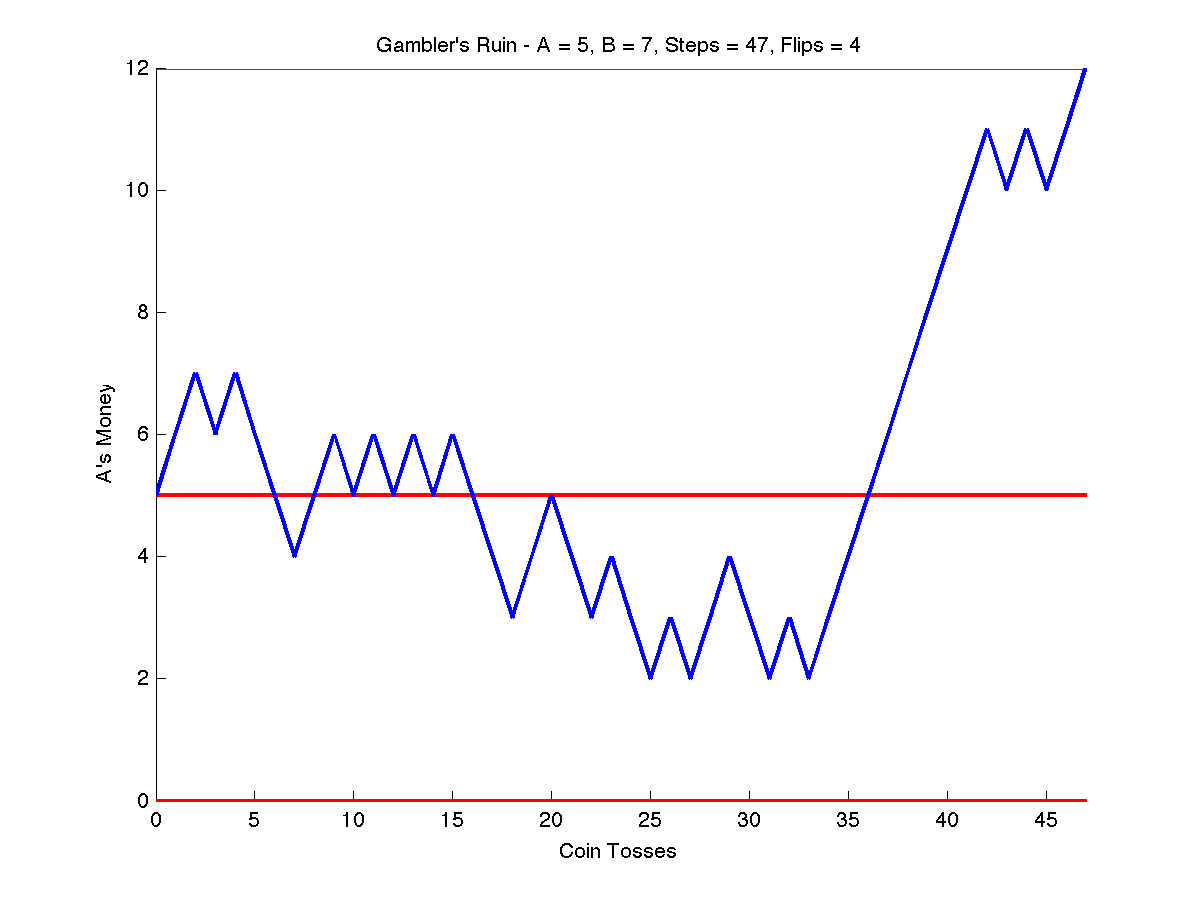
\includegraphics[width=0.7\linewidth]{images/gamblerruinnew}
\caption{}
\label{fig:gamblerruinnew}
\end{figure}

\end{frame}
%=========================================================================== %

\begin{frame}[fragile]
	\frametitle{Gambler's Ruin}
\begin{framed}
\begin{verbatim}
A=20;B=100;p=0.47
Rn=c(A)
Total=A+B

while(A>0)
  {
  UnifVal=runif(1)

  if(UnifVal <= p)
     {
     A = A+1; B =B-1
     }else{A=A-1;B=B+1}
  Rn=c(Rn,A)
  if(A==Total){break}
  }
\end{verbatim}
\end{framed}
\end{frame}

%=========================================================================== %

\begin{frame}
	\frametitle{Gambler's Ruin}
\begin{itemize}
\item We can construct a plot to depict the gambler's ongoing fortunes in the game. 
\item We use a \texttt{for} loop, that implements the game, recording the duration of the game each time. 
\item The duration of each game is the dimension of the \texttt{Rn} vector, i.e. \texttt{length(Rn)}.
\end{itemize}


\end{frame}
%=========================================================================== %
\begin{frame}[fragile]
	\frametitle{Gambler's Ruin}
\begin{framed}
\begin{verbatim}
A.ini=20;B=100;p=0.47;M=1000
RnDist=numeric();Total=A+B
for (i in 1:M)
    {
    Rn=numeric();    Rn[1]=A;    A=A.ini
    while(A>0)
        {
        UnifVal=runif(1)

        if(UnifVal <= p)
            {
            A = A+1; B =B-1
            }else{A=A-1;B=B+1}
        Rn=c(Rn,A)
        if(A==Total){break}
        }
    RnDist=c(RnDist,length(Rn))
    }
\end{verbatim}
\end{framed}
\end{frame}
%==================================================================== %
\begin{frame}[fragile]
\frametitle{Distribution of Durations}
\textbf{Simpler Approach}
\begin{framed}
\begin{verbatim}
A=50;B=200;p=0.47
GAME = A+cumsum(sign(p-runif(1000)))

which(GAME==0)[1]
 # [1] 402

which(GAME==(A+B))[1]
 # [1] NA
\end{verbatim}
\end{framed}

\end{frame}
%=========================================================================== %
\begin{frame}[fragile]
	\frametitle{Gambler's Ruin}
\begin{framed}
	\begin{verbatim}
T1 <- Sys.time()
A <- 50 ; B<- 100 ; p <- 0.48
M=50000
Duration = c()
GamblerWins = c()
for (i in 1:M)
{
	GAME = A+cumsum(sign(p-runif(20000)))
	Duration <- c(Duration, which(GAME==0)[1])
	GamblerWins <- c(GamblerWins, which(GAME==(A+B))[1])
}
T2 <- Sys.time()
T2-T1
\end{verbatim}
\end{framed}
\end{frame}
%=========================================================================== %
\begin{frame}[fragile]
	\frametitle{Gambler's Ruin}
\begin{figure}
\centering
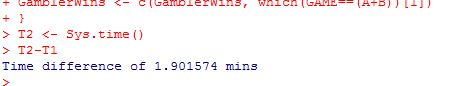
\includegraphics[width=0.9\linewidth]{images/speedgamblerruin}

\end{figure}


Quick enough, but could have faster implementation using Julia or RCPP.
\end{frame}
%=========================================================================== %
\begin{frame}[fragile]
Did the Gambler Ever Win?


	\frametitle{Gambler's Ruin}
\begin{framed}
	\begin{verbatim}
GamblerWins[!is.na(GamblerWins)]
which(!is.na(GamblerWins))

Keep <- which(!is.na(GamblerWins))
cbind(Duration[Keep],GamblerWins[Keep])

\end{verbatim}
\end{framed}

A few times! One game in every three thousand approx

\end{frame}

%===================================================================== %
\begin{frame}
	\begin{figure}
\centering
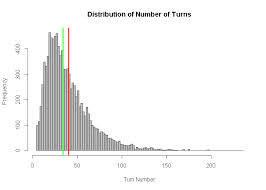
\includegraphics[width=1.1\linewidth]{images/gamblerruin}

\end{figure}

\end{frame}

\begin{frame}
	\begin{figure}
\centering
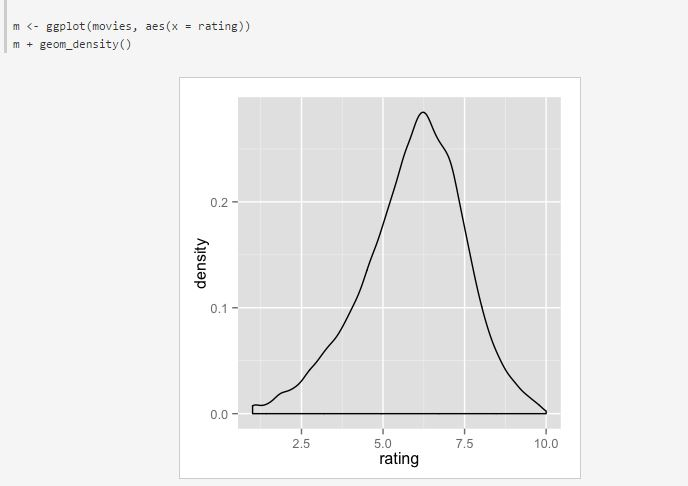
\includegraphics[width=1.05\linewidth]{images/ggplot}

\end{figure}

\end{frame}
\begin{frame}
\textbf{Kernel Density Plot}
	\begin{figure}
\centering
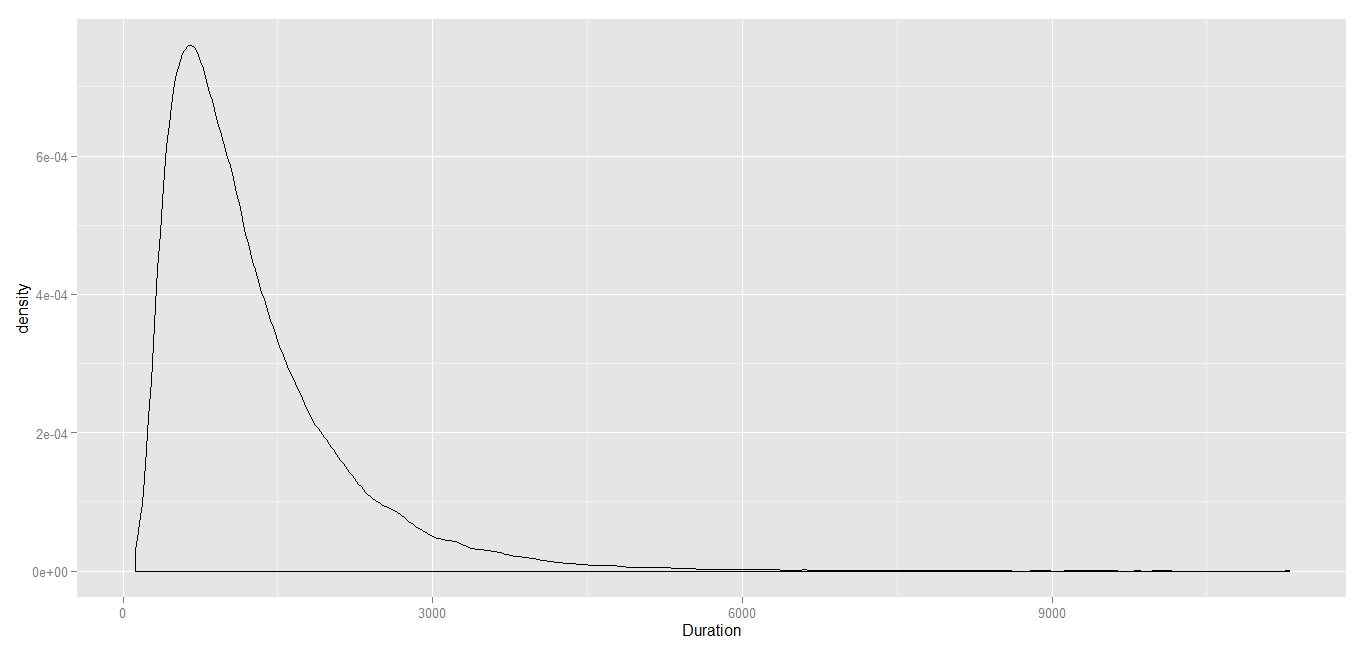
\includegraphics[width=1.1\linewidth]{images/gamblerruin-plot}

\end{figure}

\end{frame}
%=========================================================================== %
\end{document}

%- http://docs.ggplot2.org/current/stat_density.html

